\documentclass[12pt]{beamer}
\usepackage{beamerthemeHannover, graphicx, clrscode, amsmath, amssymb, multicol}
\usepackage{textcomp} \usepackage{verbatim}
\usepackage{listings}
\setbeamercolor{sidebar}{use=structure,bg=red}

\author[@dukeleto]{Jonathan "Duke" Leto\\\small{duke.leto.net\\duke@leto.net\\@dukeleto}}
\date{}
\title[PDXGit.clone()\hspace{2em}\insertframenumber/
\inserttotalframenumber]{Clone A Git Together Into Your Town}
\setbeamertemplate{navigation symbols}{} %no nav symbols

% keynote-ish
\renewcommand\sfdefault{phv}
\renewcommand\familydefault{\sfdefault}
\usetheme{default}
\usepackage{color}
\useoutertheme{default}
\usepackage{texnansi}
\usepackage{marvosym}
\definecolor{bottomcolour}{rgb}{0.32,0.3,0.38}
\definecolor{middlecolour}{rgb}{0.08,0.08,0.16}
\setbeamerfont{title}{size=\Huge}
\setbeamercolor{structure}{fg=gray}
\setbeamertemplate{frametitle}[default]%[center]
\setbeamercolor{normal text}{bg=black, fg=white}
\setbeamertemplate{background canvas}[vertical shading]
[bottom=bottomcolour, middle=middlecolour, top=black]
\setbeamertemplate{items}[circle]
\setbeamerfont{frametitle}{size=\huge}
\setbeamertemplate{navigation symbols}{} %no nav symbols

\begin{document}

\frame[t]{
    \begin{center}
            
\includegraphics[scale=0.15]{pdxgit-simantel-green}
    \end{center}
    \titlepage
}

\frame{
    \frametitle{ 
\includegraphics[scale=0.2]{pdxgit} PDX Git Together}

    \indent The monthly user group that doesn't lose your data!  \\

    \begin{huge}
        pdxgit.com
    \end{huge}

}

\frame{
    \frametitle{Infrastructure}

    \begin{itemize}
        \item Github Pages
        \item Twitter Bootstrap
        \item Font Awesome
        \item Google Groups
        \item Calagator
        \item Twitter
        \item LinkedIn
    \end{itemize}
}

\frame{
    \frametitle{History}

    \begin{itemize}
        \item GSoC Mentor Summit Oct 2010
        \item Git Together Developer Conf Oct 2010
        \item GSoC Mentor Summit Oct 2011
        \item Git Together Developer Conf Oct 2011
        \item 26. Jan 2012 pdxgit.com
        \item 1. Feb 2012 1st Meeting
        \item 27. Aug 2012 2nd Meeting (@igalko)
    \end{itemize}
}

\frame{
    \frametitle{History}

    Regular Monthly Meeting at Elemental Technologies

    \begin{itemize}
        \item 27. March 2013
        \item 24. April 2013
        \item 29. May 2013
        \item next $ \to $ 26. June. 2013
    \end{itemize}
}

\frame{
    \frametitle{Getting Free Stuff}
            
\includegraphics[scale=0.25]{free_tibet}
    \begin{itemize}
        \item Venue
        \item Food
        \item Schwag
        \item Publicity
    \end{itemize}
}

\frame{
    \frametitle{Self-Organizing Communities}
            
\includegraphics[scale=0.25]{lorenz}
    \begin{itemize}
        \item Chaos
        \item Meritocracy
        \item Transparency
    \end{itemize}
}

\frame{
    \frametitle{Community Guidelines}
            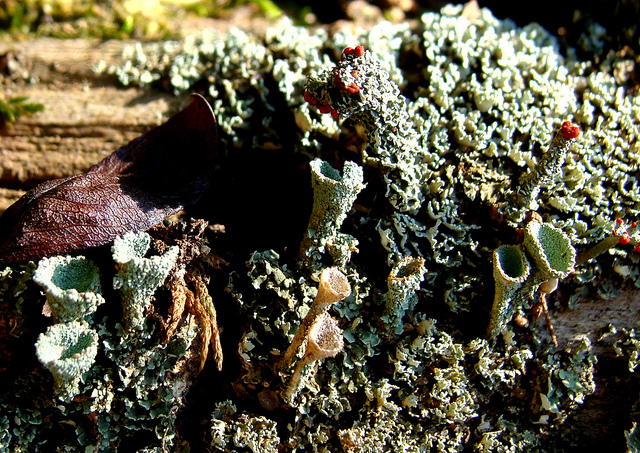
\includegraphics[scale=0.25]{lichen}
    \begin{itemize}
        \item Define  Publicly
        \item Modify  Publicly
        \item Enforce Publicly
    \end{itemize}
}

\frame{
    \frametitle{Future}
    \begin{itemize}
        \item Rotating leadership
        \item T-Shirts
        \item Stickers
        \item Focused Hackathons
    \end{itemize}
}

\frame{
    \frametitle{Checklist}

    \begin{itemize}
        \item Create a Github Org for your Clone
        \item Fork github.com/pdxgit/pdxgit.github.com
        \item Name your repo NAME.github.io (rules changed)
        \item Register a domain
        \item Change CNAME file to be your domain
        \item Configure DNS $ \to $ Github
        \item Create a Google Group
        \item Get a Twitter Account
        \item Create a LinkedIn Group
        \item ...
        \item PROFIT!
    \end{itemize}
}

\frame{
    \frametitle{How do I get involved with PDX Git Together?}
    \begin{itemize}
        \item @pdxgit
        \item pdxgit.com
        \item github.com/pdxgit
        \item pdxgit@googlegroups.com
        \item Come to the next meeting June 26th!
    \end{itemize}
}

\frame{
    \frametitle{git merge -s=social}
    \begin{center}
        \begin{itemize}
           \item @dukeleto
           \item 209.691.DUKE
           \item duke.leto.net
           \item duke@leto.net
           \item linkedin.leto.net
           \item IRC: dukeleto on Freenode, Mozilla, Perl
        \end{itemize}
    \end{center}
}

\frame{
    \frametitle{Mahalo!}
    
\includegraphics[scale=2.0]{pdxgit}
}
\end{document}
